\section{Software Entwicklung}
\begin{wrapfigure}[4]{r}[1pt]{3cm}
	\fbox{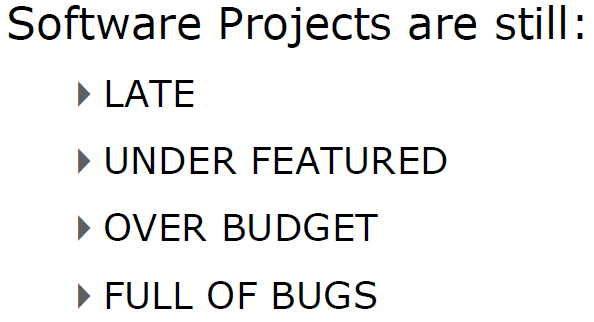
\includegraphics[width = 3cm]{images/softwareissues}}
\end{wrapfigure}
Die Softwareentwicklung ist schwierig,Hauptgrund: Komplexität.  
Ein Softwareprojekt kann sich aufgrund der Komplexität in ein Werwolf verwandeln. Dieser kann nur mit einer Silberkugel getötet werden.\\
Frederic Brooks hat dies analysiert. \\

\begin{itemize}
	\item \textit{"No Silver Bullet"} $\rightarrow$ Es gibt kein Wundermittel um komplexe Software zu entwickeln
	\item \textit{"{}Adding Manpower to a late Software project makes it later"} $\rightarrow$ Neue Leute müssen sich einarbeiten und Kommunikationsaufwand steigt. 
\end{itemize}

\subsection{Schwierigkeiten/Eigenschaften}
2 Arten von Schwierigkeiten führen zu Komplexität\\ \\
\begin{tabular}{|p{0.35\linewidth}|p{0.6\linewidth}|}
	\hline
	\textbf{Essentielle Schwierigkeiten} & Verursacht durch Komplexität des Problems \newline Essenz: Kern der Sache \\ \hline
	\textbf{Akzidentelle Schwierigkeiten} & Selbst verursacht durch falsche Methoden, Mittel \newline Akzidenz: Art der Realisierung \\ \hline\hline
	\textbf{Essentielle Eigenschaften (essential)} & Grundlegende Eigenschaften \newline \underline{Bsp.} 
	\begin{itemize}
	\item Auto muss einen Motor, Räder und Türen haben, sonst ist es kein Auto.
	\end{itemize} \\ \hline
	\textbf{Akzidentelle Eigenschaft (accidental)} & Zufällige Eigenschaft, die ein Objekt haben kann. \newline \underline{Bsp.} 
	\begin{itemize}
	\item Achtzylinder oder Vierzylindermotor
	\end{itemize} \\ \hline
\end{tabular}
\subsection{Bewältigung der Komplexität}	
		\begin{enumerate}
			\item Teile und herrsche \textit{"divide et impera"}
					\begin{itemize}
						\item Problem in Teilprobleme aufteilen
						\item Jedes Teilproblem für sich alleine lösen, alle zusammen ergeben Problemlösung
						\item Möglichst eigenständige Teile (hohe Kohäsion)
						\item Möglichst geringe Abhängigkeiten (kleine Kopplung)
					\end{itemize}
			\item Abstraktion
					\begin{itemize}
						\item Definition: Weglassen von Aspekten, die für den gegenwärtigen Zweck nicht wichtig sind.
					\end{itemize}
			\item Modelle \newline
			$\Rightarrow$ visuelle Darstellung des Sachverhalts 
					\begin{itemize}
						\item Abstraktion der realen Welt, Es gibt zwei Typen von Modellen:
                        \begin{itemize}
                        \item Design-Modelle (Lösungsdarstellung)
                        \item Domain-Modelle (Problemdarstellung)
                        \end{itemize}
					\end{itemize}
		\end{enumerate}
\subsection{Magical Number Seven}
Ein Mensch kann nur gleichzeitig 7 $\pm$ 2 Informationseinheiten im Arbeitsgedächtnis präsent halten.
\clearpage
\subsection{Vorgehen zur Softwareentwicklung}
Wenn die folgenden Schritte gleich nacheinander durchgeführt werden, spricht man von \textit{Phasen und Phasenplänen}.
	\begin{enumerate}
		\item Analyse
			\begin{itemize}
				\item Ziel: Man weiss mehr als vorher, Man weiss \textbf{\textcolor{blue}{WAS}} entwickelt werden soll.
				\item Probleme, Ideen, Anforderungen aufnehmen
				\item Erstellen eines Lasten-, Pflichtenhefts und einer Anforderungsspezifikation
				\item \textit{"doing the right things"} $\rightarrow$ Die richtigen Dinge tun
			\end{itemize}
		\item Design
			\begin{itemize}
				\item Ziel: Man weiss \textbf{\textcolor{blue}{WIE}} das Produkt entwickelt werden soll
				\item Erstellen eines \textbf{\textit{Grobentwurfs}} (Festlegung der Software-Architektur, Hilfsmittel) und \newline eines \textbf{\textit{Detailentwurfs}} (UML-Diagramme). Es entsteht noch kein Code. Nur Baupläne für die Software
				\item \textit{"doing things right"} $\rightarrow$ Die Dinge richtig tun
			\end{itemize}
		\item Implementierung
			\begin{itemize}
				\item Codieren
				\item Debuggen
				\item (Testen) $\Leftarrow$ Nicht immer!
			\end{itemize}
	\end{enumerate}

\subsection{Vorgehensmodelle (Klassisch)}
\subsubsection{Begriffe}
\begin{itemize}
	\item Ein Vorgehensmodell dient dazu die Softwareentwicklung übersichtlicher zu gestalten
	\item Schwergewichtiger Prozess $\rightarrow$ Klassische Softwareentwicklung
	\item Leichtgewichtiger Prozess $\rightarrow$ Agile Softwareentwicklung
\end{itemize}

\subsubsection{Wasserfall-Modell}
\begin{minipage}{10cm}
	\begin{itemize}
		\item lineares Vorgehensmodell
		\item nicht iterativ
		\item in Realität nicht durchführbar, da keine Rückkopplung vorhanden
		\item Freigabe beim Abschluss jeder Phase
		\item Es gibt kein zurück, alles muss beim ersten Mal richtig gemacht werden. 
	\end{itemize}
\end{minipage}
\begin{minipage}{5cm}
	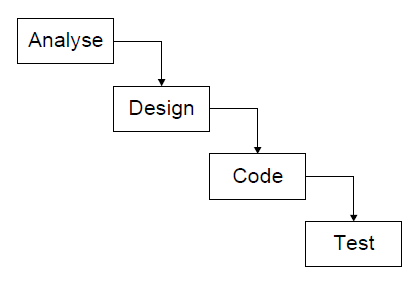
\includegraphics[width=6cm]{images/wasserfallmodell}
\end{minipage}
	
\subsubsection{Iterativer Wasserfall (Kaskade)}
	\begin{minipage}{10cm}
		\begin{itemize}
			\item Erweiterung des Wasserfalls um Korrekturschleifen
			\item In Realität durchführbar
			\item Man kann immer nur eine Phase zurück
		\end{itemize}
	\end{minipage}
	\begin{minipage}{5cm}
	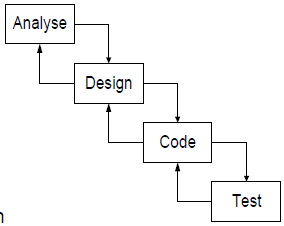
\includegraphics[width=5cm]{images/kaskade.png}	
	\end{minipage}

\subsubsection{V-Modell}
Von der deutschen Bundeswehr für ihre eigenen IT-Projekte entwickelt.\\
\begin{minipage}{8cm}
	\begin{itemize}
		\item Grundidee: Korrespondierende Tests
		\item x-Achse = Zeit
		\item y-Achse = Detaillierungsgrad
		\item Weiterentwicklung V-Modell XT,\newline
        immer projektspezifische Anpassungen nötig\newline
        (XT = Extreme Tailoring, engl. „to tailor“ = schneidern)
	\end{itemize}
\end{minipage}
\begin{minipage}{9cm}
	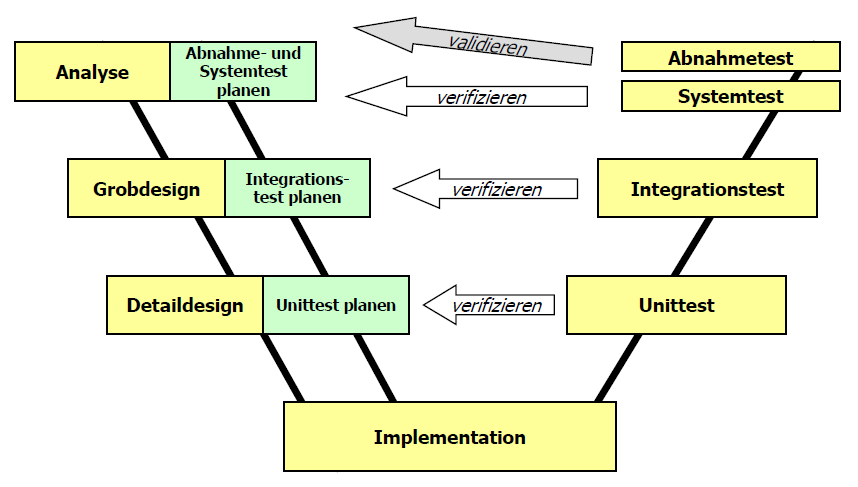
\includegraphics[width=9cm]{images/vmodell}	
\end{minipage}
\begin{wrapfigure}[4]{r}[1pt]{7cm}
	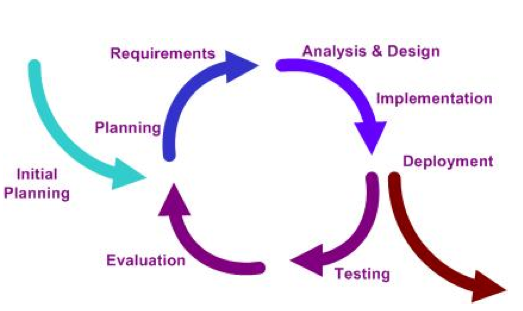
\includegraphics[width=6cm]{images/iterative_entwicklung.png}
	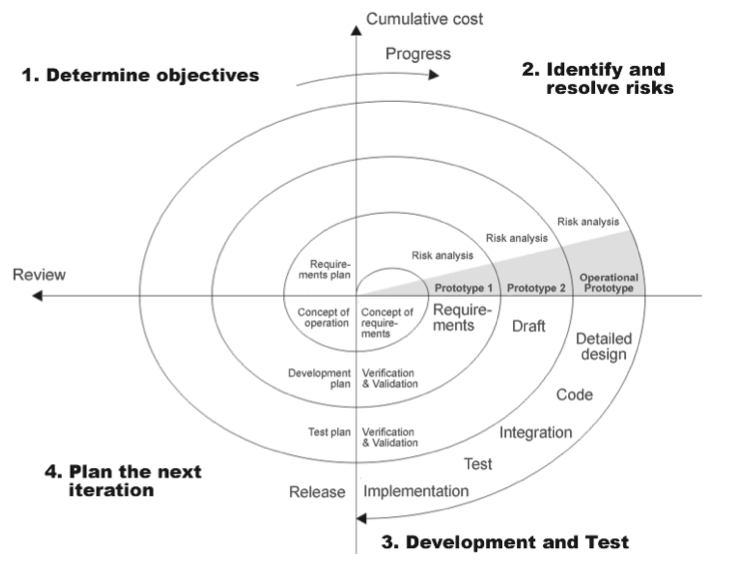
\includegraphics[width=7cm]{images/spiral_modell.png}
\end{wrapfigure}

\subsubsection{Iterative / Inkrementelle Entwicklung / Spiralmodell}
Es gibt zwei Modelle: Das Spiralmodell und RUP (Rational Unified Process).\\
\\
	\textbf{Inkrementell:}
		\begin{itemize}
			\item Resultat in Schritten entwickeln
			\item Jeder Schritt ist Teil des Endresultats \newline $\Rightarrow$ wird \underline{nicht} mehr angepasst
		\end{itemize}
	\textbf{Iterativ:}
		\begin{itemize}					
			\item Erste Version entwickeln
			\item In weiteren Schritten bessere Versionen erstellen
		\end{itemize}

\subsection{Vorgehensmodelle (Agil)}
\textit{$\Rightarrow$ Ist 3 Mal erfolgreicher als das Wasserfall-Modell}
\begin{itemize}
	\item weniger formalisiert als schwerfällige, bürokratische klassische Softwareentwicklung
	\item agil = flink, beweglich
	\item Individuen und Interaktionen gelten mehr als Prozesse und Tools
\end{itemize}

Agile Softwareentwicklung besteht aus:
\begin{enumerate}
	\item \textbf{\textit{Agile Werte:}} bilden das Fundament.
	\item \textbf{\textit{Agile Prinzipien:}} sind Handlungsgrundsätze, die auf agilen Werten basieren.
	\item \textbf{\textit{Agile Methoden:}} sind konkrete Verfahren, die sich auf agile Werte und Prinzipien stützen.
	\item \textbf{\textit{Agile Prozesse:}} sind die Zusammenfassungen angewandten Methoden.
	\\ 
\end{enumerate}
\pagebreak
\begin{multicols}{2}
\subsubsection{XP (Extreme Programming)}
\begin{minipage}{10cm}
	\begin{itemize}
		\item Bekanntester agiler Prozess
	\end{itemize}
\end{minipage}
\begin{minipage}{5cm}
	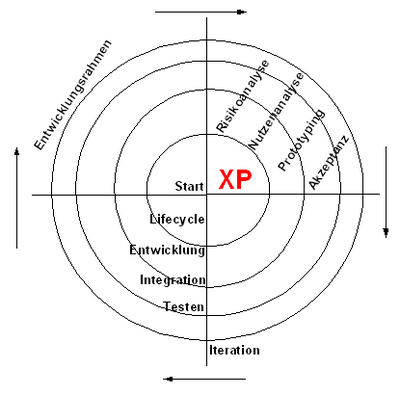
\includegraphics[width=7cm]{images/extreme_programming.png}
\end{minipage}

\subsubsection{Scrum}
$\Rightarrow$ Basiert auf sogenannten User Stories (Use Cases)\\

\begin{minipage}[l]{10cm}
	\begin{itemize}
		\item Gedränge
		\item \textit{\textbf{Basis:}} Sprints von 15-30 Tagen, in welchen vom Team eine \newline neue (brauchbarere) Softwareversion erstellt wird. 
	\end{itemize}
\end{minipage}
\begin{minipage}{10cm}
	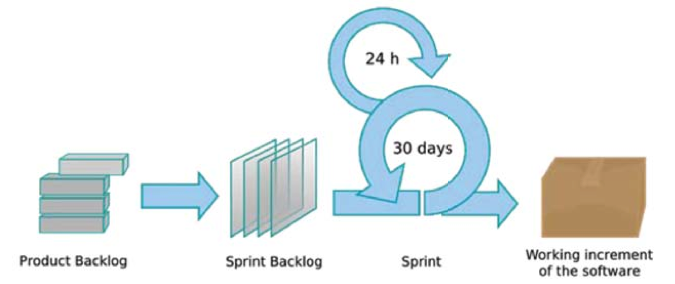
\includegraphics[width=10cm]{images/scrum.png}
\end{minipage}
\\
\end{multicols}

\subsection{Objektorientierte Softwareentwicklung (OOAD)}
\begin{minipage}[b]{13cm}
	\begin{itemize}
		\item Modelle auf allen Stufen:\textcolor{blue}{\textbf{ OO-Analyse $\rightarrow$ OO-Design $\rightarrow$ OO-Implementation}}
		\item \textit{Objekte} sind Abstraktionen von realen Dingen (Modellen)
		\item Klassen entstehen durch Gruppieren und zusammenfassen von Objekten mit gleicher Datenstruktur
		\item Gleiche Notation bei OOA, OOD, OOI
		\item Darstellung mit UML
		\item OOAD kann in jedem Vorgehensmodell verwendet werden
	\end{itemize}
	\vspace{1pt}
\end{minipage}
\newline
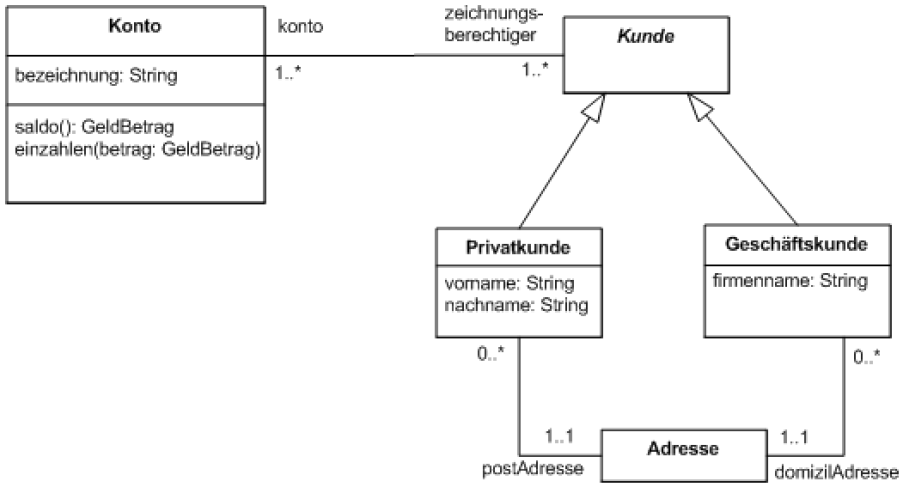
\includegraphics[width=12cm]{images/uml.png}

\begin{multicols}{2}
\subsection{Kriterien für die Wahl des Modells}
\begin{itemize}
	\item Projektgrösse
	\item Projektkomplexität
	\item Verfügbarkeit der Ressourcen
	\item Zeitpunkt von Änderungen (diskret, laufend)
	\item Qualität der Anforderungsdefinitionen
	\item Stabilität bzw. Volatilität der Anforderungen
\end{itemize}

\subsection{The Big Bang Problem bei Wasserfallmodellen}
\begin{enumerate}
	\item zuerst lange Analyse-Phase mit dem Kunden
	\item dann lange Phase für Design, Codierung und Test \newline $\rightarrow$ Kein Kundenkontakt
	\item Einführung des Systems beim Kunden $\Leftarrow$ \textcolor{blue}{\textbf{Big Bang}} 
	\item \textbf{Folge:} Hektisches Nachbessern
\end{enumerate}
$\Rightarrow$ \textit{Häufig wird dadurch das Vertrauen des Kunden zerstört.}
\end{multicols}
\clearpage